\begin{frame}
  \frametitle{Moltres}
  \textbf{What is Moltres?}
  \begin{itemize}
    \item Moltres \cite{lindsay_introduction_2018} is an open-source, MOOSE-based
      multiphysics application for modeling MSRs
	\item \gls{MOOSE} \cite{lindsay_20_2022} is an open source finite-element framework
      that supports the development of multiphysics solvers
    \item Robust and highly scalable numerical routines from PETSc
    \item Flexible coupling capabilities provided by the MOOSE Multi-App system
    \item Highly extensible and user-friendly interface for software development through
      object-oriented programming paradigm in C++ and native compatibility with other MOOSE-based
      apps
  \end{itemize}
\end{frame}

\begin{frame}
  \frametitle{Previous MSR Analyses with Moltres}
  \begin{columns}
    \hfill
    \column[t]{4cm}
      \textbf{MSRE \cite{lindsay_moltres_2017}}
      \vfill
      \begin{figure}
        \centering
	    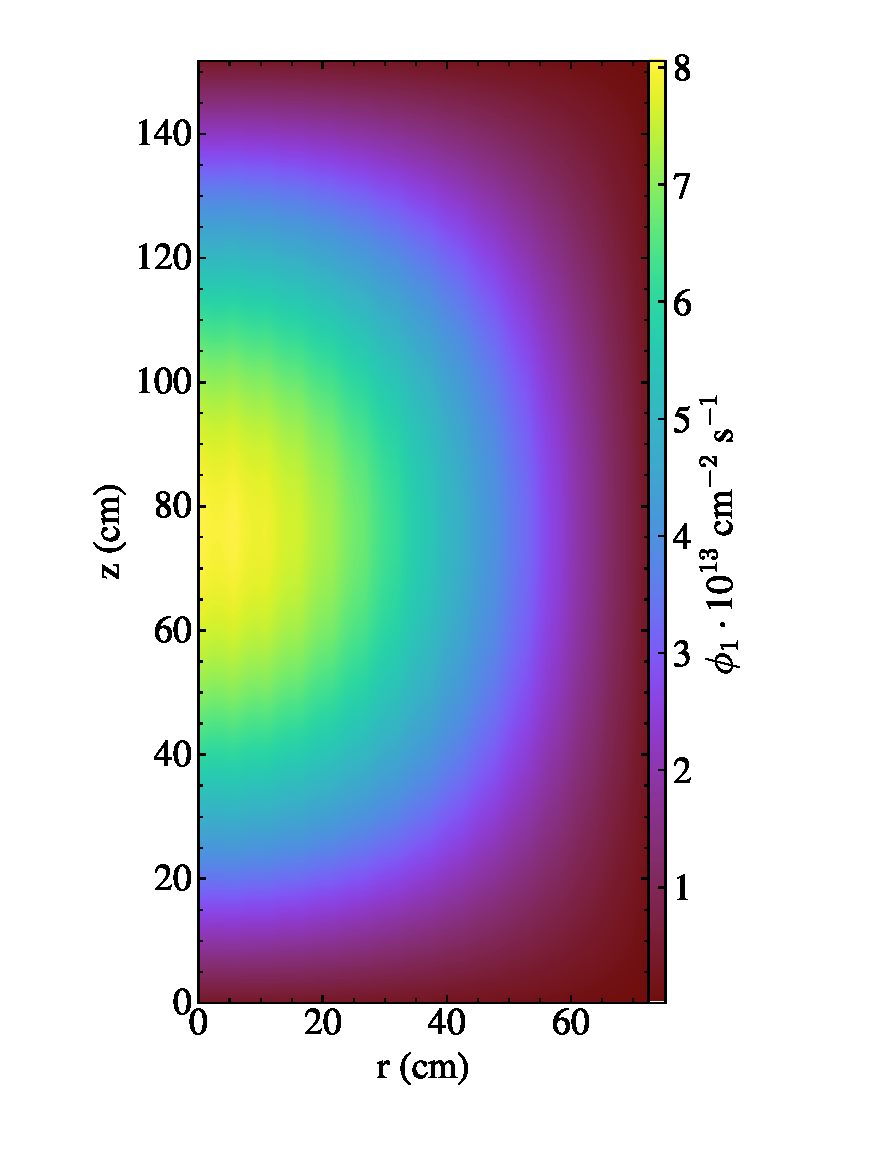
\includegraphics[width=.48\columnwidth]{../images/2d_gamma_heating_group1}
        \hfill
	    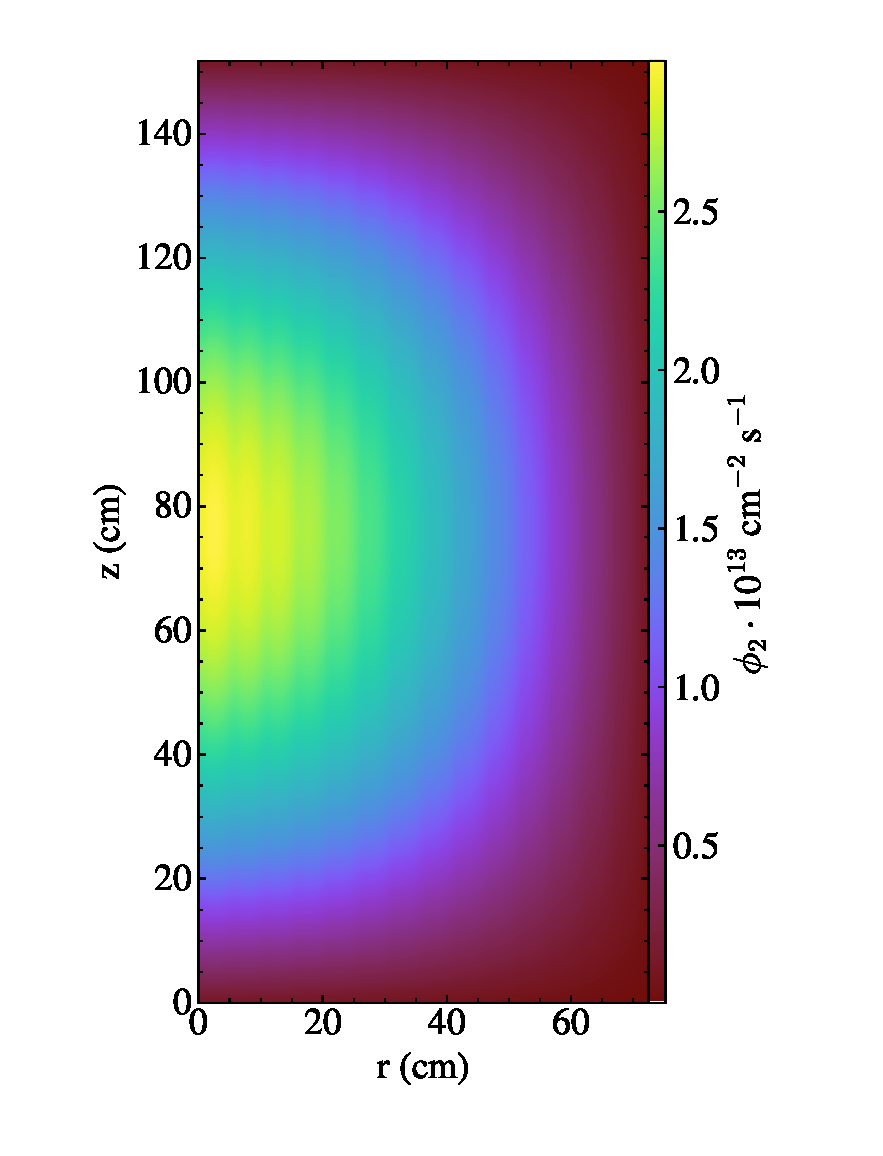
\includegraphics[width=.48\columnwidth]{../images/2d_gamma_heating_group2}
	    \caption{\footnotesize Group 1 and 2 neutron fluxes in a 2-D axisymmetric MSRE
	      model.}
      \end{figure}
    \hfill
    \column[t]{3.5cm}
      \textbf{MSFR \cite{park_advancement_2020}}
      \vfill
      \begin{figure}
        \centering
        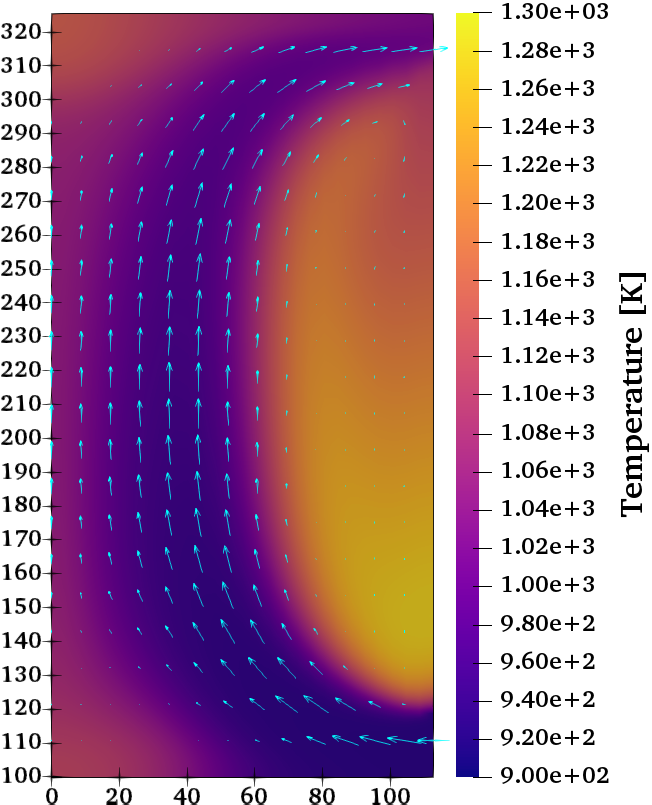
\includegraphics[width=.8\columnwidth]{images/flow-temp-plasma}
        \caption{\footnotesize Steady-state temperature distribution and salt flow velocity fields
          in a 2-D axisymmetric MSFR model.}
      \end{figure}
    \hfill
    \column[t]{3.5cm}
      \textbf{TAP MSR \cite{lee_neutronics_2020}}
      \vfill
      \begin{figure}
        \centering
        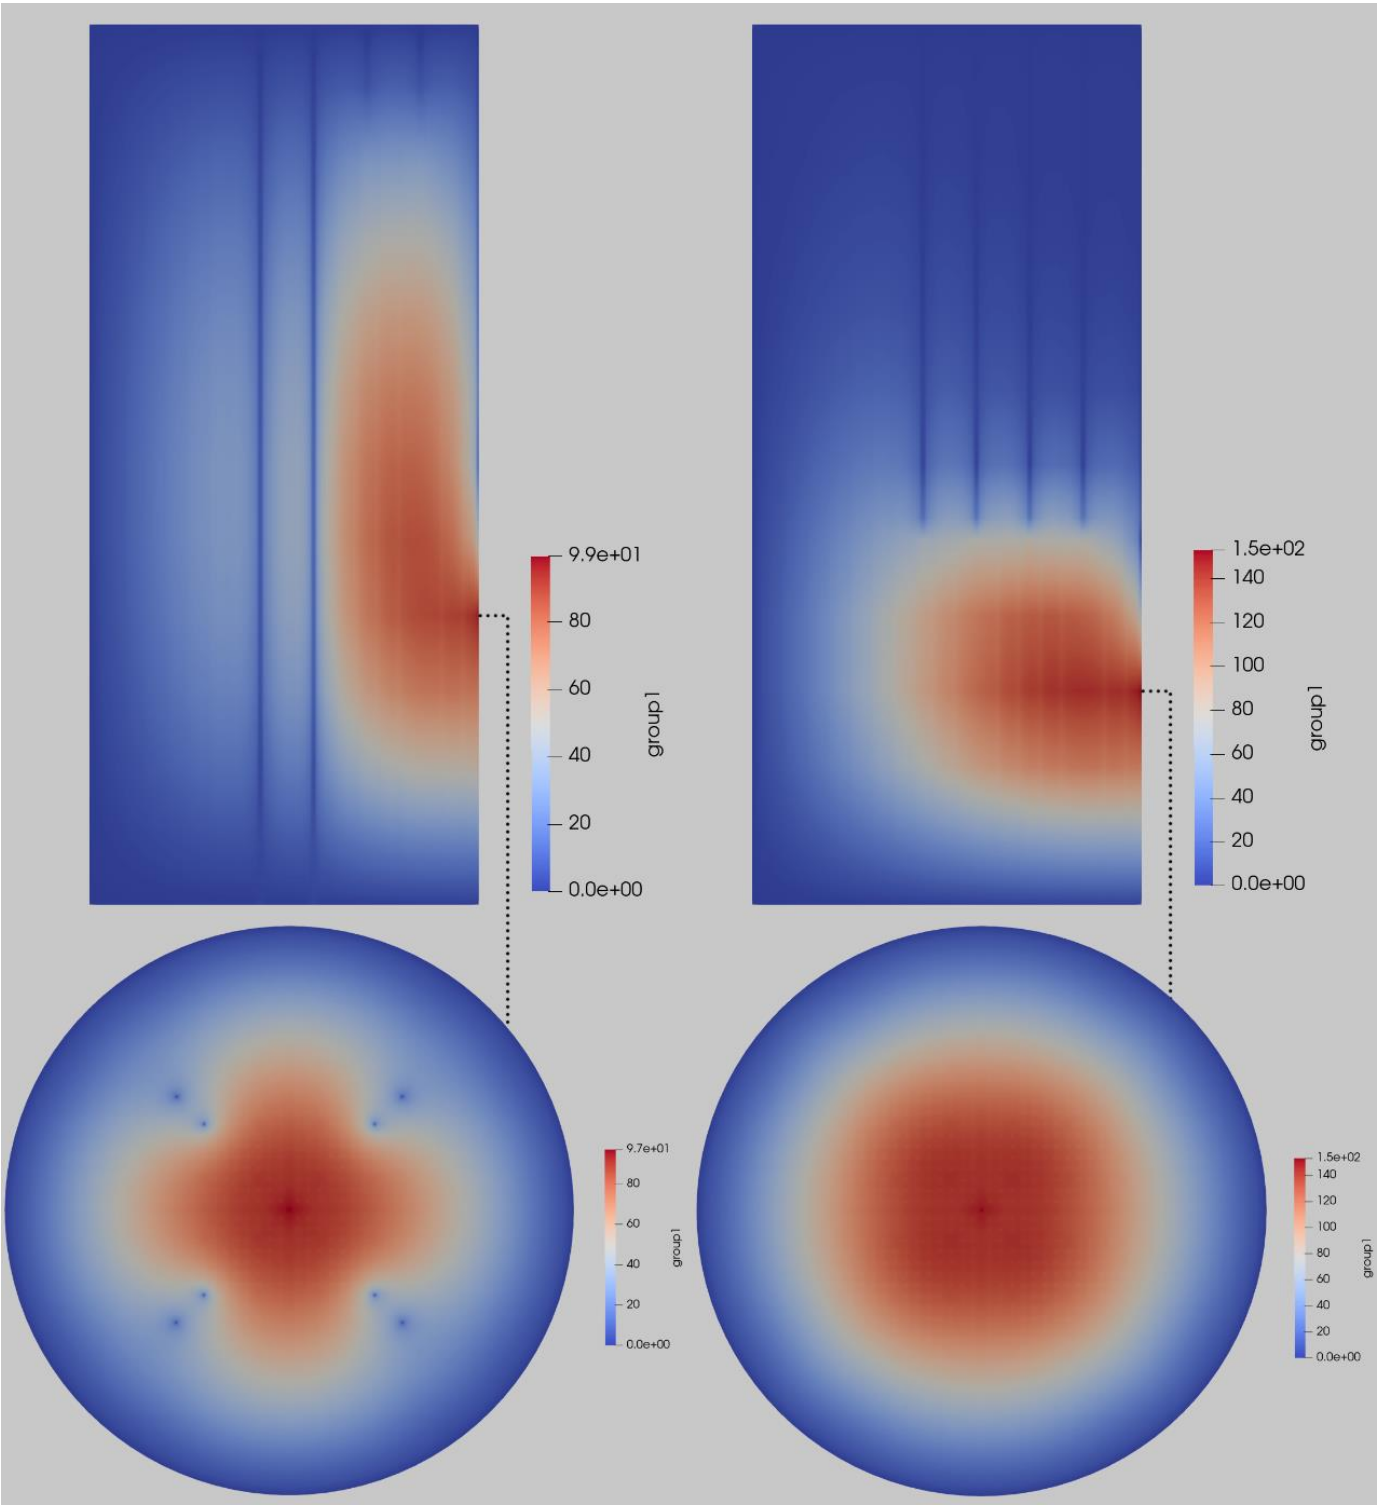
\includegraphics[width=\columnwidth]{images/tap-msr}
        \caption{\footnotesize Group 1 and 2 neutron fluxes in a 3-D TAP MSR model.}
      \end{figure}
    \hfill
  \end{columns}
\end{frame}

\begin{frame}
  \frametitle{Moltres}
  \begin{block}{\textbf{Software Capabilities for MSR Modeling}}
    \begin{itemize}
  	  \item Multigroup neutron diffusion solver
      \item Support for modeling temperature-dependence with group
        constants\footnote{Group constants refer to neutron cross section data and other
        neutronics-related material properties} generated
        from high-fidelity neutronics simulations (e.g., OpenMC)
      \item Support for coupling \gls{DNP} drift with fuel salt flow
      \item Support for out-of-core \gls{DNP} decay modeling
      \item Internal coupling with MOOSE modules for thermal-hydraulics modeling
      \item Up to 3-D modeling on unstructured meshes
    \end{itemize}
  \end{block}
\end{frame}

\begin{frame}
  \frametitle{Moltres}
  \begin{block}<1->{\textbf{Gaps in Moltres Software Development}}
    \begin{itemize}
      \item Rigorous verification and validation (V\&V) of existing multiphysics capabilities for
        MSR modeling
      \item Turbulence modeling capability for simulating high-Reynolds number flows in MSRs
    \end{itemize}
  \end{block}
  \onslide<2->{
  \textbf{Verification and Validation}

  ``Verification for single-physics codes can be achieved for many applications, but verification
  of multi-physics codes remains a difficult task, especially when the
  coupled problem is solved by iterating different solvers, ...''
  \begin{flushright}
    Tiberga et al. \cite{tiberga_results_2020}
\end{flushright}}
  \onslide<3->{
  Current V\&V status relating to previous work with Moltres:
  \begin{itemize}
    \item Limited to single-physics verification (e.g., neutronics)
    \item Significant disparities in fidelity between numerical solvers (e.g, Monte Carlo vs
      neutron diffusion)
    \item Overly complex multiphysics systems (e.g., MSFR)
    \item No validation studies yet, partly due to the lack of MSR experimental data
  \end{itemize}}
\end{frame}

\begin{frame}
  \frametitle{Moltres}
  \begin{block}<1->{\textbf{Gaps in Moltres Software Development}}
    \begin{itemize}
      \item Rigorous verification and validation (V\&V) of existing multiphysics capabilities for
        MSR modeling
      \item Turbulence modeling capability for simulating high-Reynolds number flows in MSRs
    \end{itemize}
  \end{block}
  \onslide<2->{
  \textbf{Turbulence modeling}
  \begin{itemize}
    \item The Reynolds number of salt flow in MSRs can range from $10^3$ in MSRE fuel channels
      \cite{kedl_fluid_1970} to $10^6$ in the MSFR core \cite{fiorina_modelling_2014}.
    \item Turbulent flow directly influences temperature and \gls{DNP} advection.
  \end{itemize}}
\end{frame}

\begin{frame}
  \frametitle{Moltres}
  \begin{block}<1->{\textbf{Gaps in Moltres Software Development}}
    \begin{itemize}
      \item Rigorous verification and validation (V\&V) of existing multiphysics capabilities for
        MSR modeling
      \item Turbulence modeling capability for simulating high-Reynolds number flows in MSRs
    \end{itemize}
  \end{block}
  \begin{block}<2->{\textbf{Proposed Work}}
    \begin{itemize}
      \item \textbf{Verify and Validate Existing Multiphysics Coupling Capabilities in Moltres}
      \item \textbf{Implement a RANS-based Turbulence Model in Moltres}
    \end{itemize}
  \end{block}
\end{frame}
